\documentclass[aspectratio=169]{beamer}

\usetheme{Madrid}
\usecolortheme{default}

\usepackage{amsmath}
\usepackage{graphicx}

\title{ECE 251: Floating-Point Architecture}
\subtitle{Week 08 Notes}
\author{Rob Marano}
\date{Spring 2026}

\begin{document}

\frame{\titlepage}

\begin{frame}{Overview}
\begin{itemize}
    \item Transitioning to \textbf{Chapter 3} of the textbook.
    \item Previous focus was exclusively on the \textbf{Integer Data Type} (signed/unsigned).
    \item Real-world engineering requires processing fractional decimal values.
    \item We explore:
    \begin{itemize}
        \item The limitations of Fixed-Point logic.
        \item The \textbf{IEEE 754 Protocol} standard.
        \item How MIPS handles numbers using \textbf{Coprocessor 1 (FPU)}.
        \item Hardware implementation and FPU pipelining.
        \item Immediates and literal constraints in ISA.
    \end{itemize}
\end{itemize}
\end{frame}

\begin{frame}{1. The Decimal Dilemma: Fixed vs. Floating Point}
\begin{itemize}
    \item Physical memory and CPU registers have a strict 32-bit limit.
    \item \textbf{The Fixed-Point Approach:} Divide the 32 bits evenly (e.g., 16 bits integer, 16 bits fraction).
    \begin{itemize}
        \item \textbf{Pro:} Hardware simplicity. Traditional integer \texttt{add} works natively.
        \item \textbf{Con:} Extreme range limitation. Maximum computable macro-scale number is $32,767$.
        \item Lacks the vast dynamic range needed for physics simulations or graphics rendering.
    \end{itemize}
\end{itemize}
\end{frame}

\begin{frame}{The Floating-Point Protocol (IEEE 754)}
\begin{itemize}
    \item Standardized by IEEE in 1985 to maximize dynamic range and precision.
    \item Uses scientific notation: hardware dynamically ``floats'' the decimal point.
    \item \textbf{Binary Floating Point Formula:} $(-1)^{s} \times (1 + \text{Fraction}) \times 2^{(\text{Exponent} - \text{Bias})}$
\end{itemize}
\vspace{0.2cm}
\begin{center}
    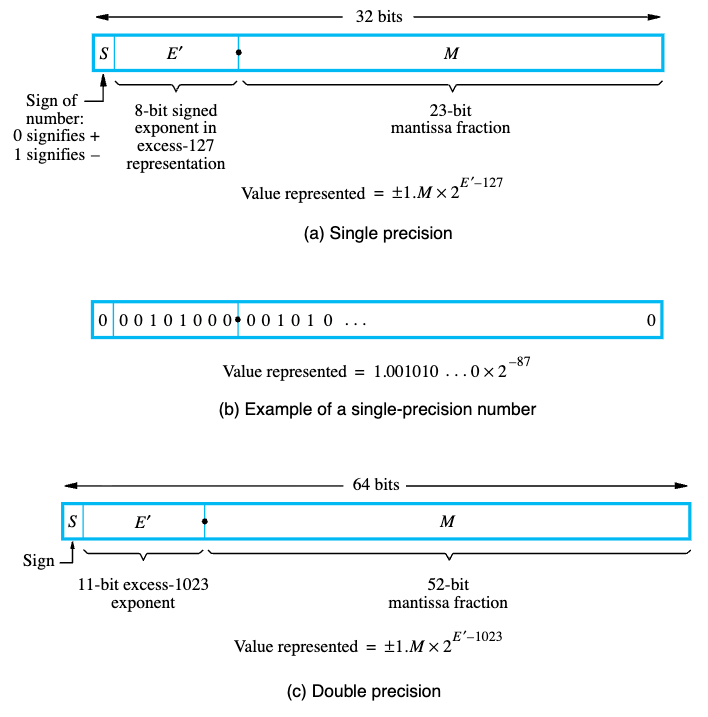
\includegraphics[width=0.65\textwidth,height=0.45\textheight,keepaspectratio]{images/hamacher_fig9_26.png}
\end{center}
\end{frame}

\begin{frame}{MIPS Single Precision (32-bit) Format}
\begin{center}
Mathematically packed into three distinct fields:
\vspace{0.5cm}

\begin{tabular}{|c|c|c|}
    \hline
    \textbf{Sign (1 bit)} & \textbf{Exponent (8 bits)} & \textbf{Fraction / Mantissa (23 bits)} \\
    \hline
    Bit 31 & Bits 30--23 & Bits 22--0 \\
    \hline
\end{tabular}

\vspace{0.5cm}
\end{center}
\begin{itemize}
    \item \textbf{Sign:} \texttt{1} = negative, \texttt{0} = positive.
    \item \textbf{Exponent:} Uses a Bias of $+127$ for Single Precision.
    \item \textbf{Mantissa:} The precise fractional magnitude.
\end{itemize}
\end{frame}

\begin{frame}{2. Hardware Segregation: Coprocessor 1 (The FPU)}
\begin{itemize}
    \item FPU arithmetic requires significantly different logical gates than integer math.
    \item Combining logic into one monolithic ALU creates massive processor bottlenecks.
    \item MIPS formally delegates decimal math to a secondary chip: \textbf{Coprocessor 1 (FPU)}.
    \item \textbf{FPU Register File:} Maintains its own separate array of 32 physical registers (\texttt{\$f0} through \texttt{\$f31}).
    \begin{itemize}
        \item \textbf{Single Precision:} 32 bits per register natively.
        \item \textbf{Double Precision:} Pairs adjacent registers (e.g., \texttt{\$f0}/\texttt{\$f1}) for 64-bit payloads.
    \end{itemize}
\end{itemize}
\end{frame}

\begin{frame}{Specialized FPU Instructions}
\begin{itemize}
    \item Standard MIPS integer instructions (\texttt{add}, \texttt{lw}) cannot physical access the FPU.
    \item Requires dedicated Coprocessor commands (\texttt{.s} for single, \texttt{.d} for double):
    \vspace{0.2cm}
    \begin{itemize}
        \item \textbf{Loading/Storing:} \texttt{lwc1 \$f0, 0(\$a0)} (Load to Coprocessor 1)
        \item \textbf{Arithmetic:} \texttt{add.s \$f0, \$f1, \$f2} (Floating-Point Addition)
        \item \textbf{Moving Data:} \texttt{mfc1 \$t0, \$f12} (Move \textit{From} Coprocessor 1)
    \end{itemize}
\end{itemize}
\vspace{0.2cm}
\begin{center}
    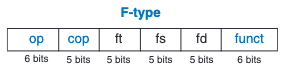
\includegraphics[width=0.65\textwidth,height=0.45\textheight,keepaspectratio]{images/harris_fig6_35.png}
\end{center}
\end{frame}

\begin{frame}{3. IEEE 754 Standard Deep Dive}
\begin{itemize}
    \item \textbf{Biased Notation for Exponents:} FPU applies $+127$ bias instead of Two's Complement. Ensures exponents are strictly positive binary integers for fast comparator logic.
    \item \textbf{Normalized Mantissas:} The leading \texttt{1} is implicitly hidden (\texttt{1.xxxxx}), providing 24 bits of effective precision in a 23-bit space.
    \item \textbf{Special Values:} \texttt{0} (Exp=0, Frac=0) and \textbf{NaN} (Exp=255, Frac$\neq$0).
\end{itemize}
\begin{center}
    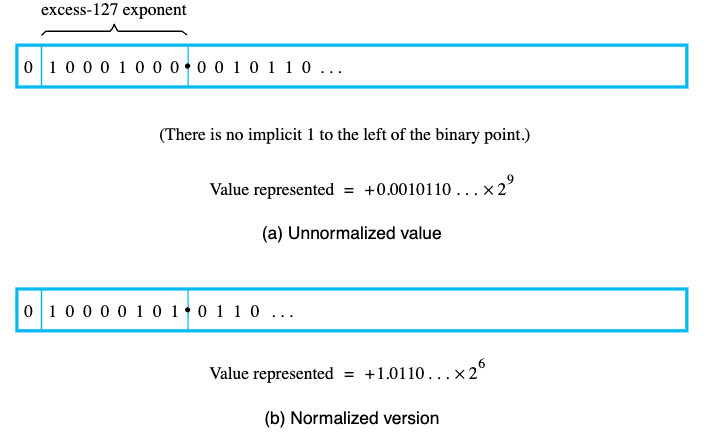
\includegraphics[width=0.6\textwidth,height=0.5\textheight,keepaspectratio]{images/hamacher_fig9_27.png}
\end{center}
\end{frame}

\begin{frame}{Example: Decimal to Single Precision}
\textbf{Problem:} Convert $-0.75_{10}$ to IEEE 754 Single Precision.
\vspace{0.3cm}
\begin{enumerate}
    \item \textbf{Binary Fraction:} $-0.75_{10} = -3/4 = -0.11_{2}$.
    \item \textbf{Normalize:} $-1.1_{2} \times 2^{-1}$.
    \item \textbf{Sign Field:} Negative $\rightarrow$ \texttt{1}.
    \item \textbf{Exponent Field:} True is $-1$. Add bias: $-1 + 127 = 126 \rightarrow$ \texttt{01111110}.
    \item \textbf{Mantissa Field:} Drop hidden \texttt{1}, pad fraction \texttt{1} with zeros $\rightarrow$ \texttt{100 0000...}
\end{enumerate}
\vspace{0.3cm}
\textbf{Final 32-bit Code:} \texttt{1 01111110 10000000000000000000000} (\textbf{\texttt{0xBF400000}})
\end{frame}

\begin{frame}{Example: IEEE 754 to Decimal}
\textbf{Problem:} Convert \texttt{0xC1480000} back to base-10 decimal.
\vspace{0.3cm}
\begin{enumerate}
    \item \textbf{Hex to Binary:} \texttt{1100 0001 0100 1000 0000 0000 0000 0000}
    \item \textbf{Slice:} \texttt{1 | 10000010 | 10010000000000000000000}
    \item \textbf{Sign:} \texttt{1} $\rightarrow$ Negative ($-$).
    \item \textbf{Exponent:} $130 - 127 (\text{bias}) = 3 \rightarrow 2^{3}$.
    \item \textbf{Mantissa:} Append hidden \texttt{1.} $\rightarrow 1.1001_{2}$.
    \item \textbf{Combine:} $-1.1001_{2} \times 2^{3} \rightarrow -1100.1_{2}$.
    \item \textbf{Convert:} $-(8+4+0.5) = \mathbf{-12.5_{10}}$.
\end{enumerate}
\end{frame}

\begin{frame}{4. Literal Values in ISA Design}
\begin{itemize}
    \item \textbf{Literals/Immediates:} Hardcoded numbers inside code (e.g., \texttt{addi \$t0, \$t0, 4}).
    \item \textbf{''Make the Common Case Fast'':} Small constants make up over $50\%$ of operands. MIPS limits the immediate field purely to 16 bits via the \textbf{I-Type Format} to avoid memory fetches.
    \item \textbf{The 32-bit Alternative:} What if we need to load \texttt{0x003D0900}? We must use a two-instruction macro:
    \begin{itemize}
        \item \texttt{lui \$s0, 0x003D} (Loads \texttt{0x003D} to upper 16-bits).
        \item \texttt{ori \$s0, \$s0, 0x0900} (ORs \texttt{0x0900} to lower 16-bits).
    \end{itemize}
\end{itemize}
\end{frame}

\begin{frame}{5. Microarchitectural Hardware Implementation}
\begin{columns}
\begin{column}{0.45\textwidth}
\begin{itemize}
    \item \textbf{Integer Datapath:} $\sim$ 1 cycle.
    \item \textbf{FPU Datapath:} Must pipe sequentially:
    \begin{enumerate}
        \item \textbf{Alignment} (Shifting)
        \item \textbf{Execution} (Fraction Add)
        \item \textbf{Normalization}
        \item \textbf{Rounding} (IEEE limit)
    \end{enumerate}
    \item \textbf{Bottleneck:} FPUs natively \textbf{pipeline} across 4 to 6 cycles constraint.
\end{itemize}
\end{column}
\begin{column}{0.55\textwidth}
    \begin{center}
        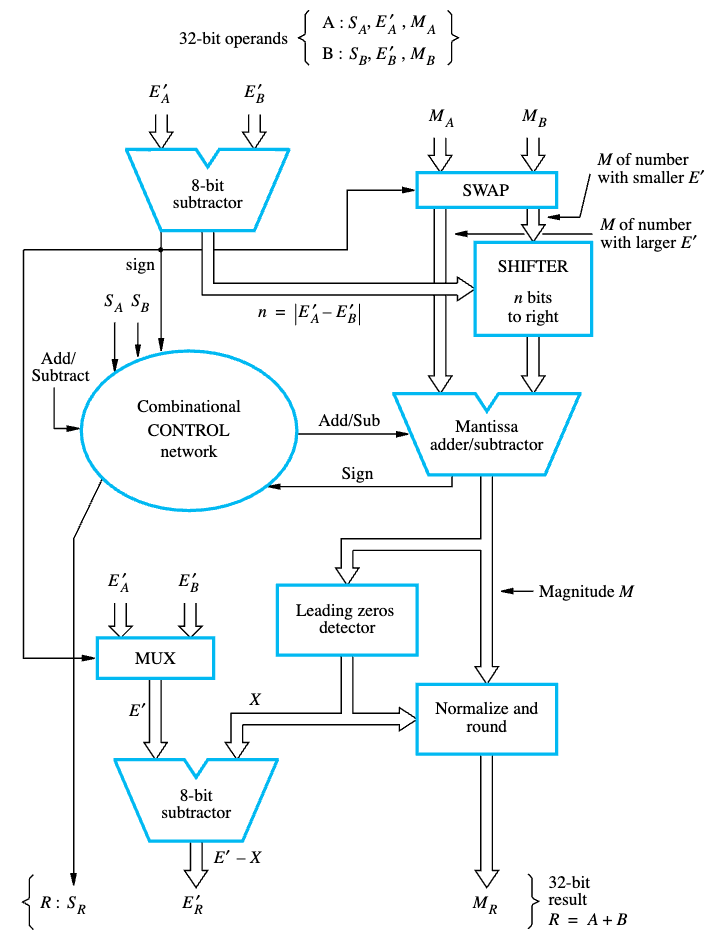
\includegraphics[width=\textwidth,height=0.65\textheight,keepaspectratio]{images/hamacher_fig9_28.png}
    \end{center}
\end{column}
\end{columns}
\end{frame}

\begin{frame}{Example: FPU Pipeline Addition Trace}
\begin{columns}
\begin{column}{0.4\textwidth}
\begin{itemize}
    \item \textbf{Trace:} $7.875_{10} + 0.1875_{10}$
    \item \textbf{Step 1-2:} Unpack Exponent/Fraction.
    \item \textbf{Step 3-4:} Compare Exponents and \textbf{Align} the fractional mantissas.
    \item \textbf{Step 5:} Perform fractional \textbf{Execution} (Addition).
    \item \textbf{Step 6:} \textbf{Normalize} the shifted result.
    \item \textbf{Step 7-8:} \textbf{Round} and pack back into 32-bit register format.
\end{itemize}
\end{column}
\begin{column}{0.6\textwidth}
    \begin{center}
        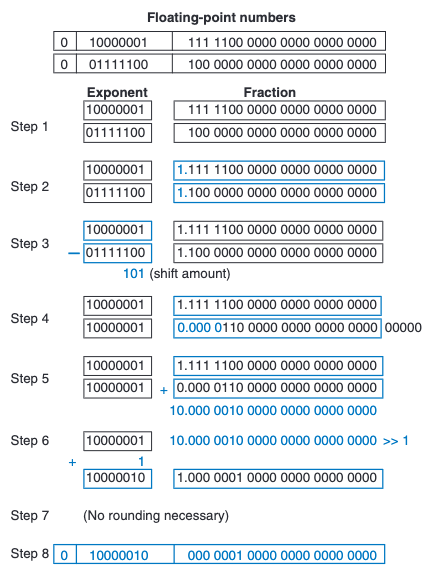
\includegraphics[width=\textwidth,height=0.75\textheight,keepaspectratio]{images/harris_fig5_29.png}
    \end{center}
\end{column}
\end{columns}
\end{frame}

\begin{frame}[fragile]{6. The Quake III Inverse Square Root Hack}
\begin{itemize}
    \item How do we approximate $\frac{1}{\sqrt{x}}$ without halting the CPU for 20+ cycles?
    \item \textbf{The MIPS Trick:} Move the float to an integer register, bit-shift right, and subtract from a magic constant!
\end{itemize}
\vspace{0.2cm}
\begin{center}
\begin{minipage}{0.9\textwidth}
\begin{verbatim}
# Move float bits from FPU ($f12) into CPU Integer Register ($t0)
mfc1  $t0, $f12          

# i = 0x5f3759df - ( i >> 1 );
srl   $t1, $t0, 1        # Bit-shift right by 1
lw    $t2, magic         # Load magic number (0x5f3759df)
sub   $t0, $t2, $t1      # Integer subtraction
\end{verbatim}
\end{minipage}
\end{center}
\vspace{0.2cm}
\begin{itemize}
    \item \textbf{Why it works:} IEEE 754 structure is inherently logarithmic.
    \item Shifting bits right (\texttt{i >> 1}) mathematically scales the float exponent by 0.5 (calculating $x^{-0.5}$).
    \item Subtracting from \texttt{0x5f3759df} negates the target exponent, approximates the fractional curve, and perfectly re-aligns the $+127$ bias!
\end{itemize}
\end{frame}

\begin{frame}{Conclusion}
\begin{itemize}
    \item Decimal values break classical fixed-point architectures.
    \item The global IEEE 754 standard introduces computational limits and brilliant bias formatting to squeeze massive range out of 32 bits.
    \item Physical processor frequency dictates that these complex derivations be outsourced to a segregated, pipelined Coprocessor unit.
\end{itemize}
\vspace{1cm}
\begin{center}
    \textbf{Questions and Hardware Review}
\end{center}
\end{frame}

\end{document}
